

\chapter{Results and Discussion}

The results of the benchmarks were aggregated by mean over at least five repeated runs. The aggregated results can be found in Table \ref{TABLE:RESULTS} at the end of this chapter. Take special note of the extremely long runtimes for the ANN runs which include the interaction list processing. What follows is a graphical analysis of the benchmark results. First comes an overview of the results, followed by a more detailed breakdown of the search methods into the components and comparison over different fill types and fill percentages.

Figure \ref{FIG:runtimeall} shows the total runtime of the frNN search over various fill types. Each color represents a different a search method. The cell linked-list method ({\itshape CLL}) is in blue, the ANN library with interaction list processing in green, and the ANN library but without list processing (ANN-NoList, or {\itshape ANN-NL}) in orange. Note that there are no results for ANN for some test cases as the processing times for these cases exceeded reasonable values. The scattering in the x-axis does not have a meaning and is only to prevent overlapping of data points.

\begin{figure}[h]
	\centering
	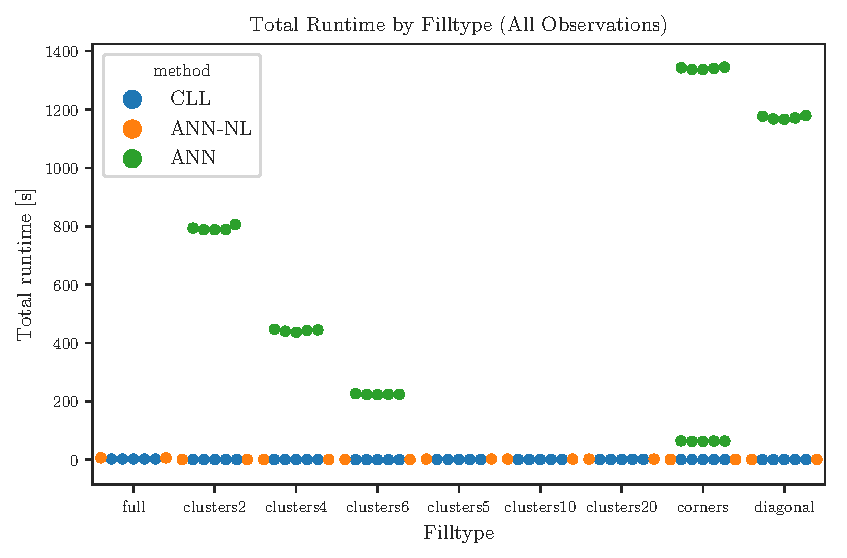
\includegraphics[width=\textwidth]{figures/totalruntime_all.pdf}
	\caption{Mean total runtime grouped by fill type.}
	\label{FIG:runtimeall}
\end{figure}

It is immediately apparent that the ANN runs take much longer than the other methods. In Figure \ref{FIG:runtimenoann}, ANN has been removed from the plot and only the CLL and ANN-NL runs are shown. With a more reasonable y-axis scale, we see that runtimes for ANN-NL are still significantly longer than CLL runtimes in almost all cases. In other words, the CLL method is faster and outputs the results in the correct format, while the ANN search itself takes longer and does not include the processing step.

\begin{figure}[h]
	\centering
	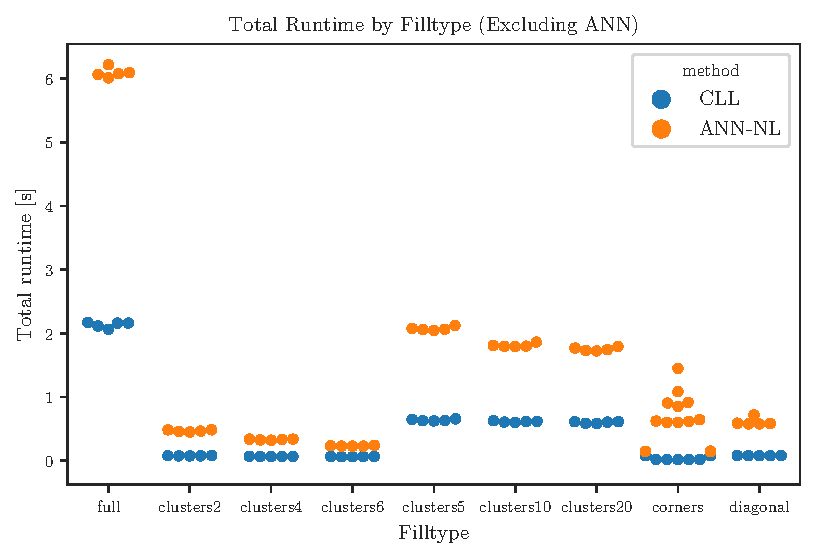
\includegraphics[width=\textwidth]{figures/totalruntime_noann.pdf}
	\caption{Total process runtime grouped by fill type, excluding ANN}
	\label{FIG:runtimenoann}
\end{figure}

\begin{figure}[h]
	\centering
	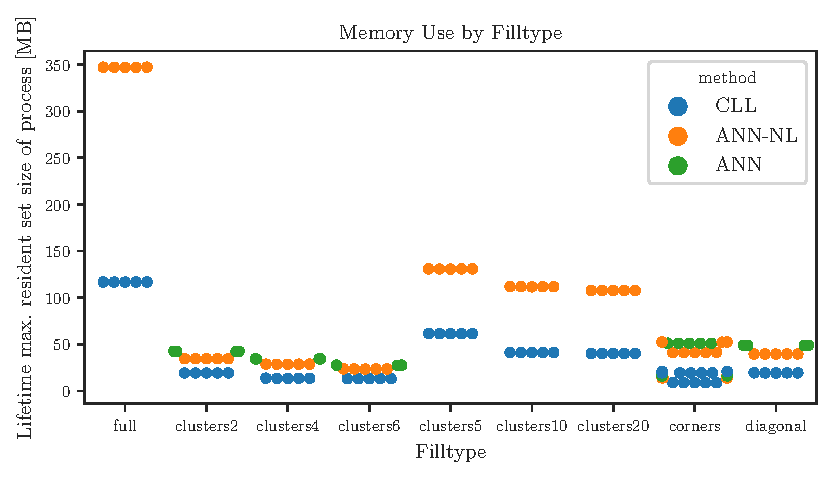
\includegraphics[width=\textwidth]{figures/memory_all.pdf}
	\caption{Mean maximum memory use grouped by filltype.}
	\label{FIG:memoryall}
\end{figure}

\pagebreak{}

Comparing memory use in Figure \ref{FIG:memoryall}, the ANN and ANN-NL methods are similar, with ANN-NL slightly below ANN. This is not surprising, as the memory requirements for the list generation are small compared to the kd-tree structure. However, the CLL method uses about one-half of the amount of memory that the ANN methods use.

Figure \ref{FIG:splitruntimeann} makes the expense of the list generation very clear by splitting the total runtime of the ANN search method into the search time and the list processing time. The runtimes are grouped by fill type and are averaged over different fills. The search time is made up of the time to find the number of neighbors of each point ({\itshape tksearch}, blue) and the time to retrieve the neighbors from the data structure ({\itshape tfrsearch}, yellow). The list processing time ({\itshape tprocessing}) is shown in a separate chart.  Note the different scales of the y-axes. 

\begin{figure}[h]
	\centering
	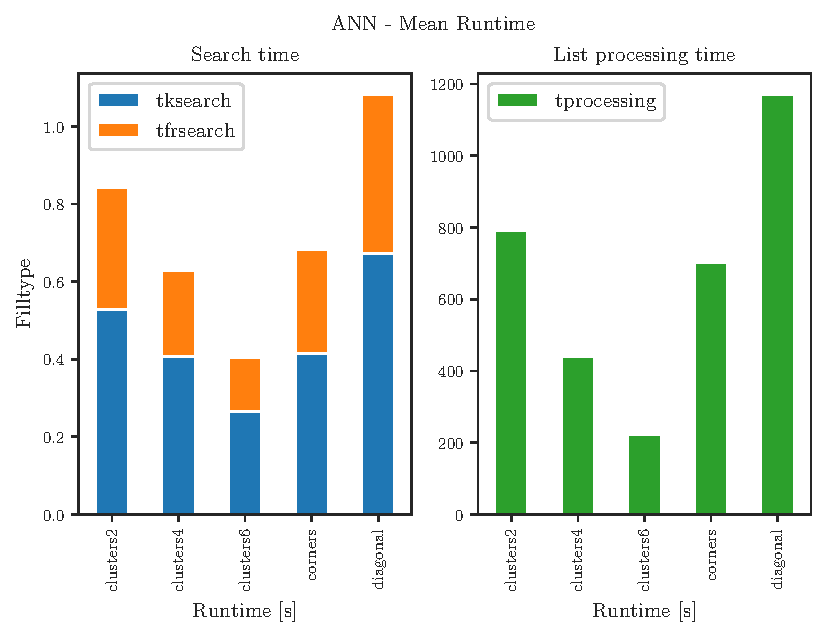
\includegraphics[width=\textwidth]{figures/ann_splitruntime.pdf}
	\caption{Total process runtime of the ANN search method split into search time (left) and interaction list processing time (right).}
	\label{FIG:splitruntimeann}
\end{figure}

The search times lie in a range of about 0.4 to 1.2 seconds. About $\frac{2}{3}$ of the search time is spend determining the neighbors and $\frac{1}{3}$ of it is spent retrieving the neighbors. The list processing times range from 200 to 1200 seconds, i.e. generating the interaction pair lists is 100x more expensive than the search itself. Therefore, for the ANN search method to be at all reasonable, either a significant performance increase in the list processing or a different approach that does not require the interaction lists at all must be found. 

\section{Effect of Fill}
\label{SECTION:ANALYSISFILL}

The fill was expected to have a significant effect on the runtime and memory use. Figure \ref{FIG:runtimefilltypes} shows, for each search type, the runtimes sorted from left to right by increasing fill percentage. For the ANN and ANN-NL methods, the total time is split into the neighbor search, neighbor retrieval, and list processing times. Some bars are very small due to the y-axis scale. See Table \ref{TABLE:RESULTS} for the actual values. The runtimes for the test cases with 11\% fill are also discussed in more detail in the next section. 

For the ANN search type, some results are not available as these benchmarks did not complete in reasonable time. Furthermore, the search and retrieval times are so small compared to the list processing time that they are not visible in the bar chart. Here it is only apparent that the fill percentage has the largest overall effect on the runtime. Going from 2\% to 11\% fill leads in the best case to a 3.5-fold increase in the total runtime. In the worst case, the total runtime for 11\% fill is 21 times that of the case with 2\% fill. With 51\% fill, the runtime exceeds 8 hours. Although not as extreme as the fill, the fill type also clearly has a large effect. This is discussed in more detail in Section \ref{SECTION:ANALYSISFILLTYPE}.

For CLL and ANN-NL the total runtime also generally increases with increasing fill percentage. From 11\% to 51\% fill, the CLL method runtime increases about 7.8 times and the ANN-NL method increases 4.1 times. From 51\% to 100\% fill, the CLL method runtime increases about 3.5 times and the ANN-NL method increases 3.3 times. Therefore we could say that the CLL method is probably more sensitive to the fill percentage in sparsely filled domains ($< 50\%$ fill) than the ANN-NL search. However, in all cases examined here, the CLL method was still significantly faster than ANN-NL even at very low fills. For example, at 2\% fill, ANN-NL requires 0.15s while CLL requires only 0.02s and and already outputs the interaction pair lists as required by the current SPH implementation.

\begin{figure}[h]
	\centering
	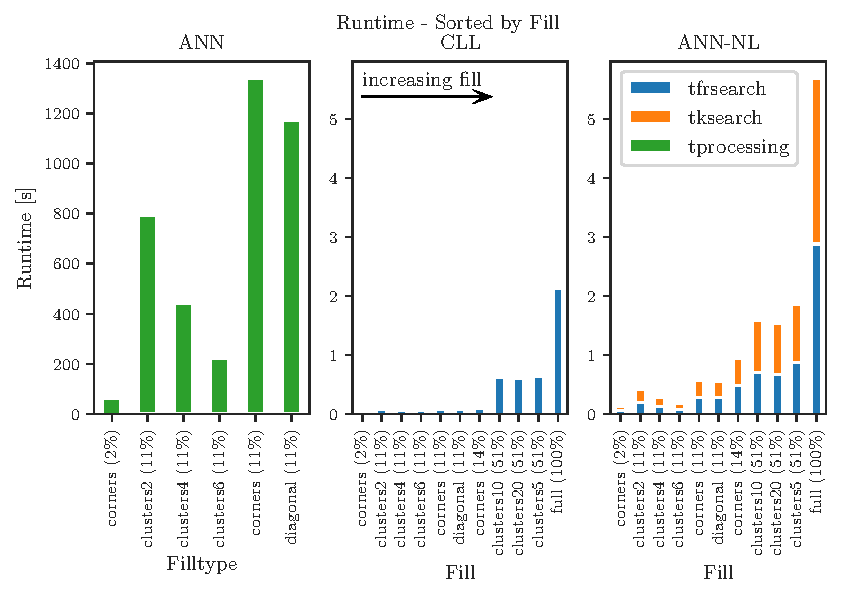
\includegraphics[width=\textwidth]{figures/runtime_filltypes.pdf}
	\caption{Total process runtimes sorted by fill percentage, for different search methods} 
	\label{FIG:runtimefilltypes}
\end{figure}

Figure \ref{FIG:memoryfilltypes} shows the maximum memory use of the search processes for each search type, with the fill again increasing from left to right. The memory use generally shows the same trends as the runtime results. Here as well CLL has an advantage over the ANN and ANN-NL search methods. The difference between ANN and ANN-NL is nowhere near as great as in the runtime. ANN-NL unsurprisingly requires less memory than ANN, as it does not have to store the interaction lists. But its clear that the bottleneck in the list generation step for high fills is in processing power and not memory.

\begin{figure}[h]
	\centering
	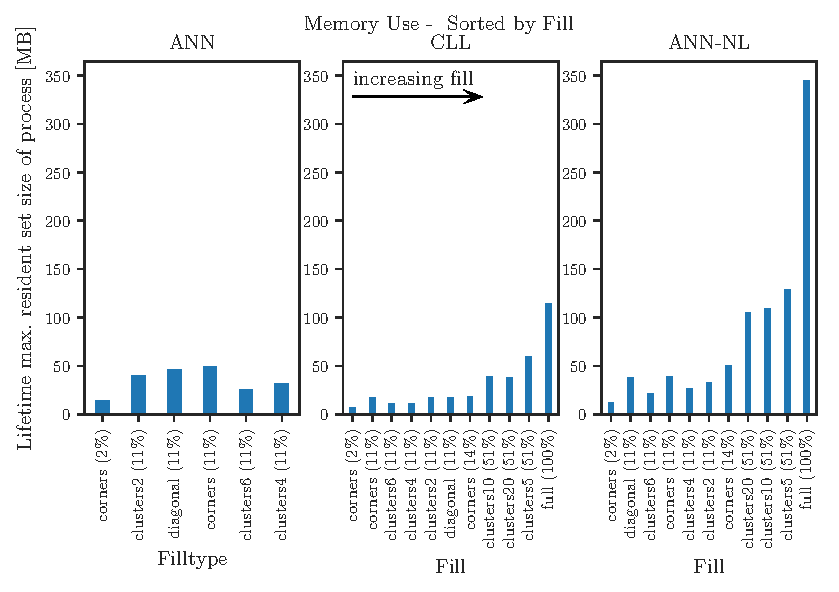
\includegraphics[width=\textwidth]{figures/memory_filltypes.pdf}
	\caption{Maximum memory use sorted by fill percentage, for different search methods} 
	\label{FIG:memoryfilltypes}
\end{figure}

\section{Effect of Fill Type}
\label{SECTION:ANALYSISFILLTYPE}

This section discusses the effect of effect of various particle distributions. For example, there could be only a few larger clusters in the domain, or many small clusters. The effect of vertical/horizontal or angled cluster boundaries is also examined briefly. In the following, various fill types are compared for the same amount of particles in the domain. The test cases following in this section are made up of between 27648 and 29424 points in the domain, which equates to between 11.06 and 11.70 percent fill.

Figure \ref{FIG:runtimefill11} shows the total runtime for each filltype for each search method. Only the results with a fill of 11\% are shown, and the total time is split into neighbor search, neighbor retrieval, and list processing time for ANN and ANN-NL search methods. The runtime on the y-axis of the figure is cut off at 1.5 seconds to facilitate comparison between the search methods. To see total runtimes for the ANN method refer back to Figure \ref{FIG:runtimefilltypes}.

A note on the cluster sizes for the 5 fill types shown here: The {\itshape corners} fill type has the largest clusters of all fill types, as all points are arrayed in two clusters in opposite corners of the domain. The {\itshape diagonals} follows close behind, with the particles distributed in 8 clusters. Then, for the {\itshape clusters} cases, the {\itshape clusters2} fill type has the largest clusters, {\itshape clusters4} is in-between, and {\itshape clusters6} has the smallest clusters. Refer also to the figures in Section \ref{SECTION:TESTCASES}.

\begin{figure}[h]
	\centering
	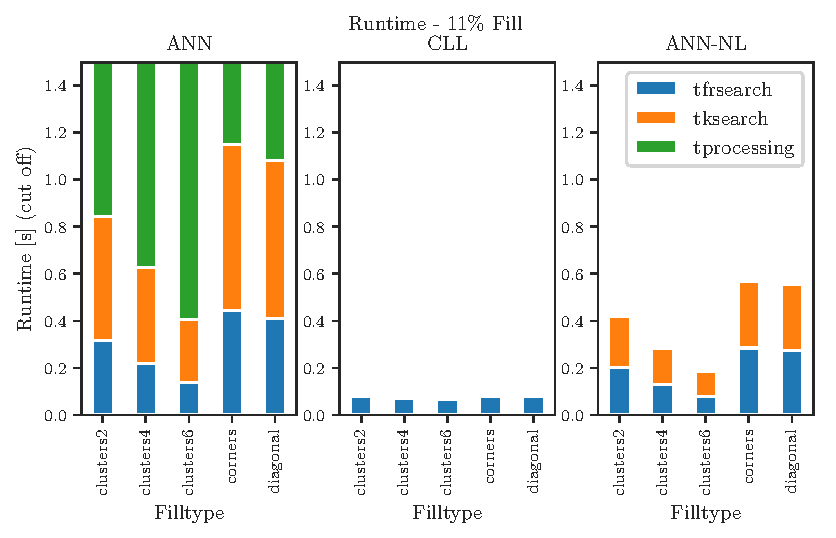
\includegraphics[width=\textwidth]{figures/runtime_fill11.pdf}
	\caption{Total process runtimes for various fill types at 11\% fill.}
	\label{FIG:runtimefill11}
\end{figure}

The total runtime of the CLL method is not significantly affected by the fill type. The results for the ANN methods do show an effect. It can be seen in the {\itshape clusters} cases that smaller clusters generally lead to a decrease in the runtime.

There is no significant difference between the {\itshape diagonal} and {\itshape corners} fill types. However, it was expected that the diagonal case would faster than the corners case, based on the difference in cluster sizes. So there could in fact be a negative impact on performance when the cluster boundaries are not orthogonal or parallel to the domain bounds. However, proving this definitively requires more test cases.

Interestingly, when ignoring the list processing time, ANN-NL method is significantly faster than the ANN method. This was not expected, as the only difference between the ANN and ANN-NL methods is the commenting-out of the source code for the list processing. Without closer examination, this is chalked up to some compiler optimizations or similar effects.

In Figure \ref{FIG:memoryfill11} the memory use of the search methods for each fill type for a fill of 11\% are shown. The trend again is aligned closely with the results for the runtime, with smaller clusters reducing the memory required and little difference between the {\itshape diagonal} and {\itshape corners} fill types. ANN-NL requires a bit less memory than ANN, as expected. For the CLL search method, there is a small difference visible in the memory use for the smallest clusters ({\itshape clusters4} and {\itshape clusters6}). 

\begin{figure}[h]
	\centering
	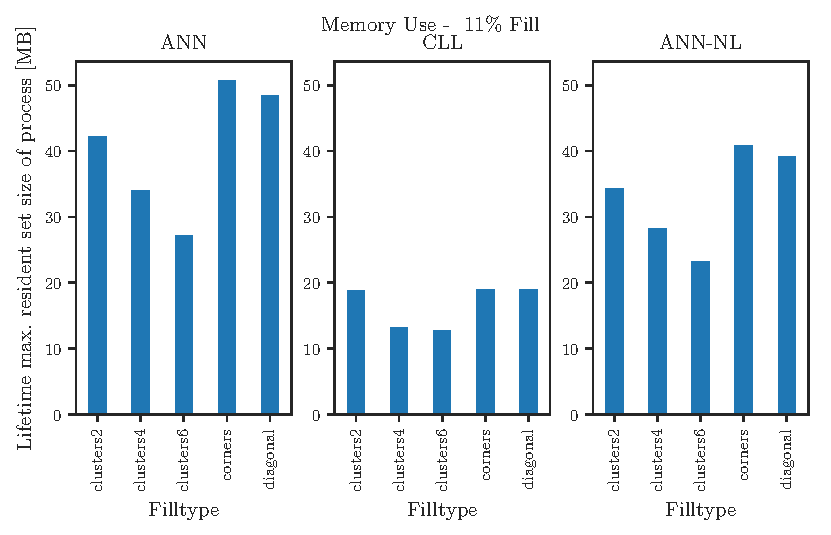
\includegraphics[width=\textwidth]{figures/memory_fill11.pdf}
	\caption{Maximum memory use for various fill types at 11\% fill.}
	\label{FIG:memoryfill11}
\end{figure}

\begin{table}[htbp]
	\centering
	\renewcommand{\arraystretch}{1.3} % Größerer Zeilenabstand
	\captionabove{All benchmarking results aggregated by mean.}
	\begin{tabular}{lllrrrrrr}
\toprule
    &      &     &  Datapts &  Memory &  $t_{frsearch}$ &  $t_{tksearch}$ &  $t_{processing}$ &  $t_{total}$ \\
fill & filltype & method &          &         &                 &                 &                   &              \\
\midrule
2 & corners & ANN &     7200 &   16.02 &            0.09 &            0.13 &             63.17 &        63.40 \\
    &      & ANN-NL &     7200 &   13.93 &            0.07 &            0.07 &              0.00 &         0.15 \\
    &      & CLL &     7200 &    8.84 &            0.00 &            0.00 &              0.00 &         0.02 \\[2.0ex]
11 & clusters2 & ANN &    27648 &   42.46 &            0.32 &            0.53 &            791.79 &       792.70 \\
    &      & ANN-NL &    27648 &   34.55 &            0.20 &            0.22 &              0.00 &         0.47 \\
    &      & CLL &    27648 &   19.18 &            0.00 &            0.00 &              0.00 &         0.08 \\
    & clusters4 & ANN &    27648 &   34.30 &            0.22 &            0.41 &            441.36 &       442.04 \\
    &      & ANN-NL &    27648 &   28.62 &            0.13 &            0.15 &              0.00 &         0.33 \\
    &      & CLL &    27648 &   13.50 &            0.00 &            0.00 &              0.00 &         0.07 \\
    & clusters6 & ANN &    27648 &   27.53 &            0.14 &            0.26 &            223.46 &       223.92 \\
    &      & ANN-NL &    27648 &   23.46 &            0.08 &            0.11 &              0.00 &         0.23 \\
    &      & CLL &    27648 &   13.03 &            0.00 &            0.00 &              0.00 &         0.07 \\
    & corners & ANN &    28158 &   51.01 &            0.45 &            0.70 &           1339.18 &      1340.39 \\
    &      & ANN-NL &    28158 &   41.14 &            0.28 &            0.28 &              0.00 &         0.62 \\
    &      & CLL &    28158 &   19.25 &            0.00 &            0.00 &              0.00 &         0.08 \\
    & diagonal & ANN &    29424 &   48.75 &            0.41 &            0.67 &           1170.92 &      1172.07 \\
    &      & ANN-NL &    29424 &   39.53 &            0.28 &            0.28 &              0.00 &         0.61 \\
    &      & CLL &    29424 &   19.27 &            0.00 &            0.00 &              0.00 &         0.08 \\[2.0ex]
14 & corners & ANN-NL &    37044 &   52.37 &            0.48 &            0.47 &              0.00 &         1.04 \\
    &      & CLL &    37044 &   20.88 &            0.00 &            0.00 &              0.00 &         0.10 \\[2.0ex]
51 & clusters10 & ANN-NL &   128000 &  111.68 &            0.71 &            0.89 &              0.00 &         1.81 \\
    &      & CLL &   128000 &   41.08 &            0.00 &            0.00 &              0.00 &         0.62 \\
    & clusters20 & ANN-NL &   128000 &  107.62 &            0.67 &            0.87 &              0.00 &         1.75 \\
    &      & CLL &   128000 &   40.04 &            0.00 &            0.00 &              0.00 &         0.60 \\
    & clusters5 & ANN-NL &   128000 &  130.79 &            0.87 &            0.99 &              0.00 &         2.07 \\
    &      & CLL &   128000 &   61.42 &            0.00 &            0.00 &              0.00 &         0.64 \\[2.0ex]
100 & full & ANN-NL &   250000 &  347.17 &            2.88 &            2.80 &              0.01 &         6.09 \\
    &      & CLL &   250000 &  116.75 &            0.00 &            0.00 &              0.00 &         2.14 \\
\bottomrule
\end{tabular}

	\label{TABLE:RESULTS}
\end{table}